\subsection{Benchmark Design}

\textsc{CentaurBench} evaluates a focal model in two roles while holding the
task and downstream worker fixed. In \emph{automation}, the focal model
receives the task prompt and produces the final deliverable. In
\emph{augmentation}, the focal model receives the same task context but
produces only an assistance text for a fixed GPT-3.5-Turbo worker. The worker
then receives the original task and the assistance text and produces the final
deliverable. A \emph{plain} condition, in which the worker receives no
assistance text, measures whether guidance improves on unaided execution.
Because the worker and worker prompt are identical across augmentation
conditions, differences in final-output quality isolate the effect of the
assistant's guidance within this simulated workflow.

We evaluate nine focal models spanning major model families; GPT-3.5-Turbo
also appears as a direct solver in automation and as the fixed worker and
unaided baseline in augmentation. The complete model versions, roles, and
judge assignments are reported in the supplementary document. The benchmark
contains seven professional tasks: counseling, market-trends analysis, menu
planning, operations research, tax preparation, travel planning, and
tutoring. The tasks vary in structure, domain knowledge, risk, and
human-facing judgment, but each specifies an observable deliverable with
explicit requirements. Full prompts and task provenance are provided in the
supplement.

\begin{figure}[t]
\centering
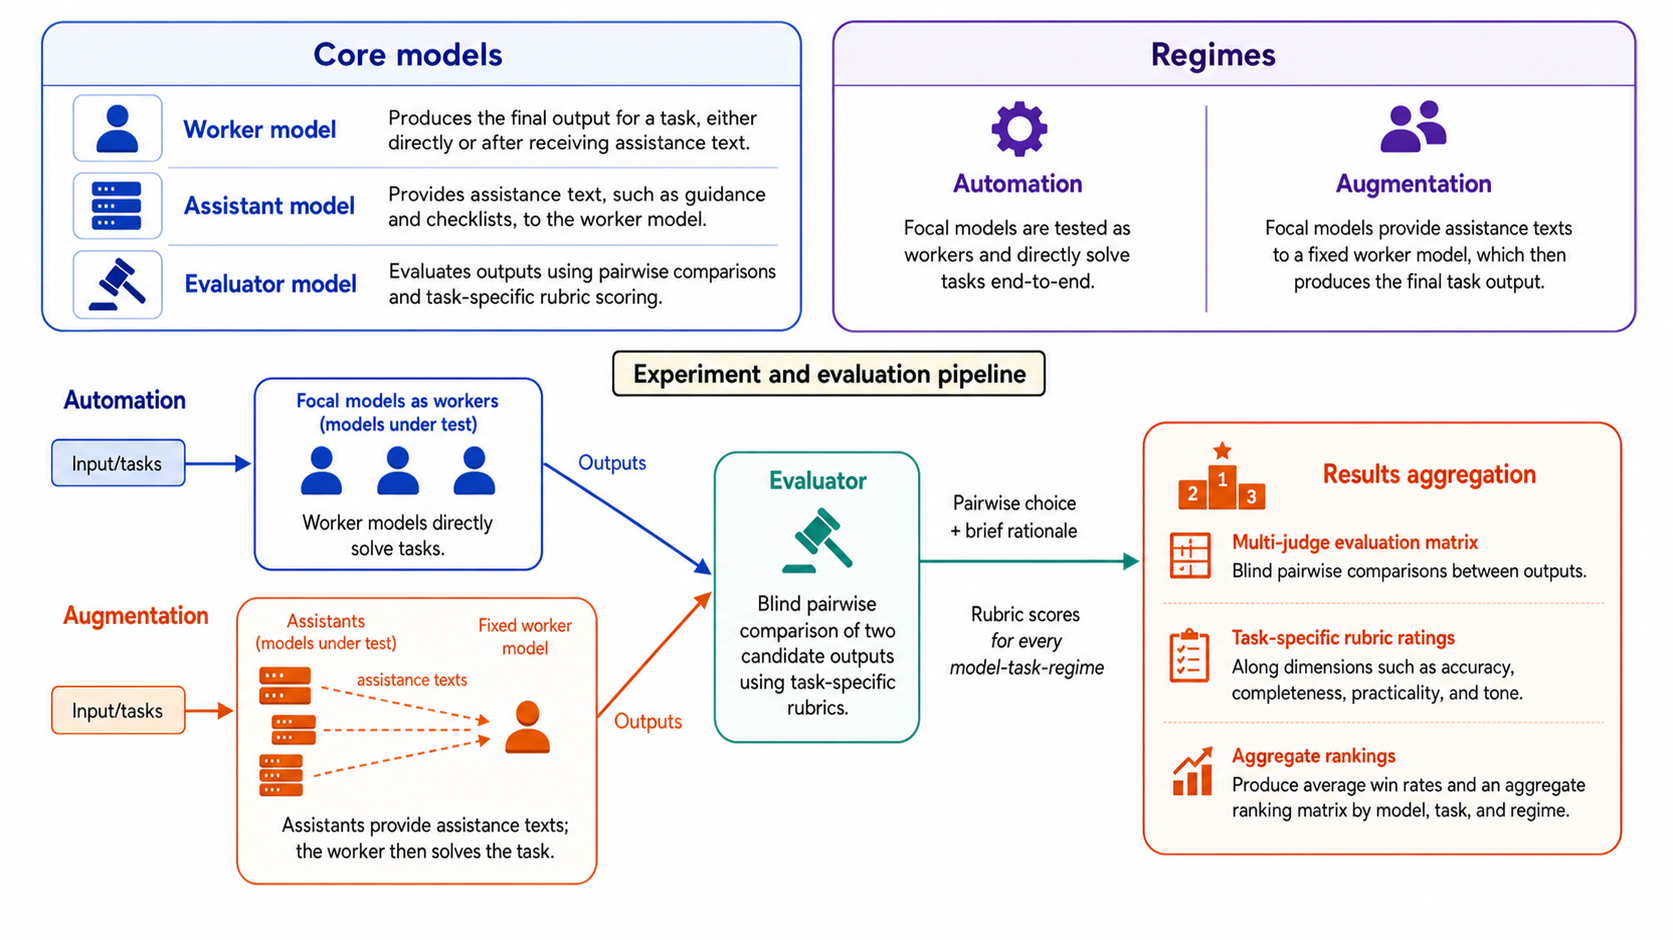
\includegraphics[width=\linewidth]{figures/methodology-final.png}
\caption{\textbf{\textsc{CentaurBench} pipeline.} The same focal models are
evaluated as direct solvers and as providers of process guidance to a fixed
worker. Blinded, rubric-guided pairwise comparisons produce task-level ranks
for each role.}
\label{fig:methodology-pipeline}
\end{figure}

\subsection{Assistance and Rubric Construction}

Each task prompt is paired with task-specific rubric dimensions that mirror
its deliverable requirements, together with five shared dimensions:
instruction following, accuracy and specificity, practical usefulness,
organization and readability, and tone/audience fit. Judges score each
dimension on a 1--10 scale before making a pairwise choice. The rubrics make
the comparison criteria explicit and preserve dimension-level diagnostics,
while pairwise choices provide the primary ranking signal
\citep{zheng2023,chiang2024}.

The assistance prompt constrains the focal model to process guidance rather
than a draft answer. It requests a requirements check, an execution plan, and
a final self-review checklist, and explicitly prohibits producing the final
deliverable. This design tests whether a model can improve another agent's
execution through planning and error prevention, not whether it can smuggle
its own solution into the worker context. It is therefore a deliberately
bounded form of augmentation; richer iterative and content-bearing assistance
remain outside the present benchmark. Verbatim prompts, rubrics, and
illustrative outputs are included in the supplement.

\subsection{Pairwise Evaluation and Ranking}

For every task, mode, and independent run, we generate one output per
candidate condition and conduct a complete round-robin tournament. Automation
and augmentation outputs are evaluated in separate tournaments. Candidate
identities are hidden and option order is randomized. Four LLM judges score
the paired outputs and select a winner, with \emph{leave-family-out} masking:
a judge is excluded whenever either candidate was generated by a model from
the judge's provider family. This reduces the most direct form of
self-preference while retaining a multi-judge panel.

For each eligible judge, pairwise choices are converted to candidate win
rates. Candidates are ranked within each task, mode, and run; ranks are then
averaged across eligible judges and ten independent runs. We report both
task-level ranks and average ranks across tasks. Cross-mode comparisons use
only the nine focal assistant models, because the unaided worker has no
corresponding assistant identity in automation.

We retain rubric scores and rationales as an audit trail and use them to check
the internal coherence of the judging procedure. Across non-tied comparisons,
the selected output has the higher mean rubric score in 99.7\% of cases.
Across 6,265 comparisons with at least two eligible judges, raw inter-judge
agreement is 71.0\% and Krippendorff's nominal
$\alpha=0.414$. Agreement is higher in automation than augmentation, indicating
that assistance outcomes are harder to judge consistently. The supplement
reports judge-level reliability, rubric--win-rate correlations, and held-out
model-family checks.
